\documentclass{ltjsarticle}

\usepackage[top=10truemm,bottom=20truemm,left=15truemm,right=15truemm]{geometry}
\usepackage{graphicx}
\usepackage{here}
\usepackage{trig}
\usepackage{listings,jvlisting}
\usepackage{luacode}
\usepackage{hyperref}
%%\topmargin =-30mm

\newcommand\DegSin[1]{\CalculateSin{#1}\UseSin{#1}}
\newcommand\DegCos[1]{\CalculateCos{#1}\UseCos{#1}}
\newcommand\DegTan[1]{\CalculateTan{#1}\UseTan{#1}}
\renewcommand{\lstlistingname}{ソースコード}

\lstset{
  frame={tb},
  breaklines=true,
  columns=[l]{fullflexible},
  numbers=left
}

\begin{luacode*}
    function to(i)
        j=i*math.pi/180
        return tostring(i).." & "..tostring(j).." & "..tostring(math.sin(j)).." & "..tostring(math.cos(j)).." & "..tostring(math.tan(j)).."\\\\"
    end
    
    function fg()
        v=""
        m="$\\vdots $ & $\\vdots $ & $\\vdots $ & $\\vdots $ & $\\vdots $ \\\\"
        for i=0,5,1 do
            v = v..to(i)
        end
        v=v..m
        for i=25,30,1 do
            v = v..to(i)
        end
        v=v..m
        for i=355,360,1 do
            v = v..to(i)
        end
        tex.sprint("\\newcommand{\\sd}{"..v.."}")
    end
\end{luacode*}
\directlua{ fg() }

\title{\LaTeX で作る三角関数表}
\author{椎木}

\begin{document}

\maketitle
\section{レギュレーション}
$0^\circ$から$5^\circ$,$25^\circ$から$30^\circ$,$355^\circ$から$360^\circ$を縦に点が3つ並ぶ記号($\vdots$)で繋ぐ表を作成する.
また,計算の為に角度の単位を変換した場合は変換後の単位も表に記す.
\section{手法の紹介}


\subsection{Excelを用いる}
Excelで計算した結果を\href{https://rra.yahansugi.com/scriptapplet/csv2tabular/}{csv2tabular}等を用いて表にする.
\begin{figure}
    \centering
    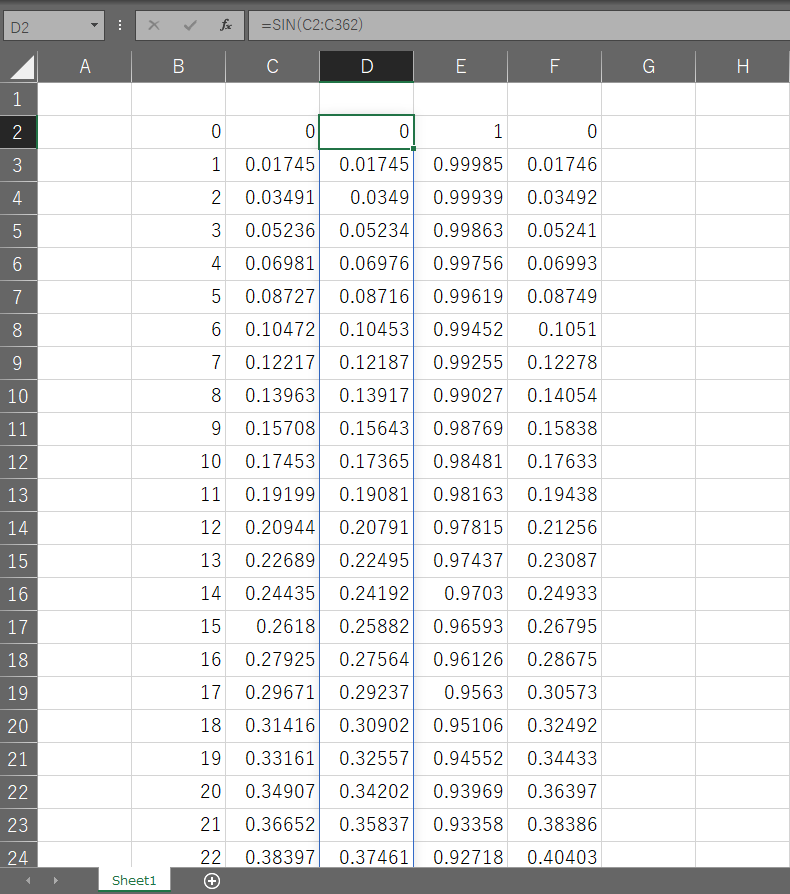
\includegraphics[scale=0.6]{ex.png}
    \caption{Excelの画面}
\end{figure}
\begin{table}[H]
    \centering
    \caption{Excelを用いた三角関数表}
    \begin{tabular}{cc|ccc}
        angle[$^\circ$]&angle[rad]&sin&cos&tan\\ \hline
        0 & 0 & 0 & 1 & 0 \\
        1 & 0.017453293 & 0.017452406 & 0.999847695 & 0.017455065 \\
        2 & 0.034906585 & 0.034899497 & 0.999390827 & 0.034920769 \\
        3 & 0.052359878 & 0.052335956 & 0.998629535 & 0.052407779 \\
        4 & 0.06981317 & 0.069756474 & 0.99756405 & 0.069926812 \\
        5 & 0.087266463 & 0.087155743 & 0.996194698 & 0.087488664 \\
        $\vdots $ & $\vdots $ & $\vdots $ & $\vdots $ & $\vdots $ \\
        25 & 0.436332313 & 0.422618262 & 0.906307787 & 0.466307658 \\
        26 & 0.453785606 & 0.438371147 & 0.898794046 & 0.487732589 \\
        27 & 0.471238898 & 0.4539905 & 0.891006524 & 0.509525449 \\
        28 & 0.488692191 & 0.469471563 & 0.882947593 & 0.531709432 \\
        29 & 0.506145483 & 0.48480962 & 0.874619707 & 0.554309051 \\
        30 & 0.523598776 & 0.5 & 0.866025404 & 0.577350269 \\
        $\vdots $ & $\vdots $ & $\vdots $ & $\vdots $ & $\vdots $ \\
        355 & 6.195918845 & -0.087155743 & 0.996194698 & -0.087488664 \\
        356 & 6.213372137 & -0.069756474 & 0.99756405 & -0.069926812 \\
        357 & 6.23082543 & -0.052335956 & 0.998629535 & -0.052407779 \\
        358 & 6.248278722 & -0.034899497 & 0.999390827 & -0.034920769 \\
        359 & 6.265732015 & -0.017452406 & 0.999847695 & -0.017455065 \\
        360 & 6.283185307 & -2.4503E-16 & 1 & -2.4503E-16 \\
        \\
    \end{tabular}
\end{table}


\newpage
\subsection{trigを用いる}
trigを用いて三角関数を計算する.
角度が$1^\circ$以上の時のコードを省略した為短く見えるが実際は27行程ある.
\begin{lstlisting}[caption=trigを用いた表のコード]
\usepackage{trig}
\newcommand\DegSin[1]{\CalculateSin{#1}\UseSin{#1}}
\newcommand\DegCos[1]{\CalculateCos{#1}\UseCos{#1}}
\newcommand\DegTan[1]{\CalculateTan{#1}\UseTan{#1}}
\begin{document}
\begin{table}[H]
  \centering
  \begin{tabular}{c|ccc}
    angle[$^\circ$]&sin&cos&tan\\ \hline
    0 & \DegSin{0} & \DegCos{0} & \DegTan{0} \\
  \end{tabular}
\end{table}
\end{lstlisting}
\begin{table}[H]
    \centering
    \caption{trigを用いた三角関数表}
    \begin{tabular}{c|ccc}
        angle[$^\circ$]&sin&cos&tan\\ \hline
        0 & \DegSin{0} & \DegCos{0} & \DegTan{0} \\
        1 & \DegSin{1} & \DegCos{1} & \DegTan{1} \\
        2 & \DegSin{2} & \DegCos{2} & \DegTan{2} \\
        3 & \DegSin{3} & \DegCos{3} & \DegTan{3} \\
        4 & \DegSin{4} & \DegCos{4} & \DegTan{4} \\
        5 & \DegSin{5} & \DegCos{5} & \DegTan{5} \\
        $\vdots $ & $\vdots $ & $\vdots $ & $\vdots $ \\
        25 & \DegSin{25} & \DegCos{25} & \DegTan{25} \\
        26 & \DegSin{26} & \DegCos{26} & \DegTan{26} \\
        27 & \DegSin{27} & \DegCos{27} & \DegTan{27} \\
        28 & \DegSin{28} & \DegCos{28} & \DegTan{28} \\
        29 & \DegSin{29} & \DegCos{29} & \DegTan{29} \\
        30 & \DegSin{30} & \DegCos{30} & \DegTan{30} \\
        $\vdots $  & $\vdots $ & $\vdots $ & $\vdots $ \\
        355 & \DegSin{355} & \DegCos{355} & \DegTan{355} \\
        356 & \DegSin{356} & \DegCos{356} & \DegTan{356} \\
        357 & \DegSin{357} & \DegCos{357} & \DegTan{357} \\
        358 & \DegSin{358} & \DegCos{358} & \DegTan{358} \\
        359 & \DegSin{359} & \DegCos{359} & \DegTan{359} \\
        360 & \DegSin{360} & \DegCos{360} & \DegTan{360} \\
        \\
    \end{tabular}
\end{table}


\newpage
\subsection{Lua言語を用いる}
Lua言語を用いて計算を行う.
純粋な$0^\circ$から$360^\circ$の表ならfor文が一回で済むため短くなる.
\begin{lstlisting}[caption=Lua言語を用いた表のコード]
\usepackage{luacode}
\begin{luacode*}
  function to(i)
    j=i*math.pi/180
    return tostring(i).." & "..tostring(j).." & "..tostring(math.sin(j)).." & "..tostring(math.cos(j)).." & "..tostring(math.tan(j)).."\\\\"
  end
    
  function fg()
    v=""
    m="$\\vdots $ & $\\vdots $ & $\\vdots $ & $\\vdots $ & $\\vdots $ \\\\"
    for i=0,5,1 do
      v = v..to(i)
    end
    v=v..m
    for i=25,30,1 do
      v = v..to(i)
    end
    v=v..m
    for i=355,360,1 do
      v = v..to(i)
    end
    tex.sprint("\\newcommand{\\sd}{"..v.."}")
  end
\end{luacode*}
\directlua{ fg() }
\begin{document}
\begin{table}[H]
  \centering
  \caption{Lua言語を用いた三角関数表}
  \begin{tabular}{cc|ccc}
    angle[$^\circ$]&angle[rad]&sin&cos&tan\\ \hline
    \sd
    \\
  \end{tabular}
\end{table}
\end{document}
\end{lstlisting}
\begin{table}[H]
  \centering
  \caption{Lua言語を用いた三角関数表}
  \begin{tabular}{cc|ccc}
    angle[$^\circ$]&angle[rad]&sin&cos&tan\\ \hline
\sd
\\
\end{tabular}
\end{table}


\newpage
\section{各手法の評価}
各手法の長所及び短所を表4にまとめた.

Excelを用いた時の長所はなによりも簡単であるところだろう.
誰にでも作れるし、時間もそれほどかからない.
Excel自体は有料ツールだが,OpenOfficeやPythonでcsvファイルを書き出すなど無料で出来る方法もあり,間違いのない方法である.
ただし,私のようにExcelが苦手だと有効数字の設定方法がよくわからず、-2.4503E-16みたいな値が出てきてしまう。

trigの長所として\LaTeX で完結するとあるが,あんなのを何回も書いているのはしんどいので,ソースコード3のようなプログラムを利用した.
\LaTeX で完結はしていないが計算自体は\LaTeX でできているし,頑張ってタイピングするのも良いと思う.
ただ,普通に有効数字が小さいと思う.

Luaの長所はきれいに書ける点が大きいかと思う.
また,精度も良く,Luaでプログラムしているため拡張性も高い.
文量に関しても多くの場合で最も短くできる.
短所は難しい上にLua\LaTeX でしか使えないところだろう.
\href{https://acetaminophen.hatenablog.com/entry/2021/06/18/022108}{pLaTeX が本格的にやばいかもという話}という記事がちょっとバズるなどして,Lua\LaTeX に注目されつつあるが,学会のテンプレート等は未だにp\LaTeX が多く,乗り換えるのも容易ではない.
こうした普及率の面からも簡単に勧められる手法とは言いにくい.
\begin{table}[H]
    \centering
    \caption{各手法の長所と短所}
    \begin{tabular}{rl|ll}
            & 手法  & 長所 & 短所 \\ \hline
        2.1 & Excel & 簡単 & \LaTeX で完結しない,Excelに詳しい必要がある \\
        2.2 & trig  & \LaTeX で完結する & 文量が多い,精度が良くない \\
        2.3 & Lua   & Lua\LaTeX で完結する,きれいに書ける & 難しい \\
  \\
  \end{tabular}
  \end{table}

\begin{lstlisting}[caption=trig用の.cppファイル]
#define REP(i,m,n) for(ll i=(ll)(m);i<(ll)(n);i++)
#define rep(i,n) REP(i,0,n)

void ptrig(int n){
  cout<< n<<" & \\DegSin{"<<n<<"} & \\DegCos{"<<n<<"} & \\DegTan{"<<n<<"} \\\\"<<endl;
}

int main() {
  rep(i,6){
    ptrig(i);
  }
  REP(i,25,31){
    ptrig(i);
  }
  REP(i,355,361){
    ptrig(i);
  }
}
\end{lstlisting}
\section{結論}
Excelを用いる手法がおすすめである.
\end{document}